\section{Data visualization}

The boxplot analyse method have been used for detecting outliers in the data set. In the boxplots below we can see that there are some outliers and some attributes where the dataset is not very detailed. The area attribute needs some stemming for correcting the data, due to a lot of zero areas. The FFMC attribute and ISI also needs stemming for cleaning up the data.

\begin{figure}
\begin{tabular}{cc}
  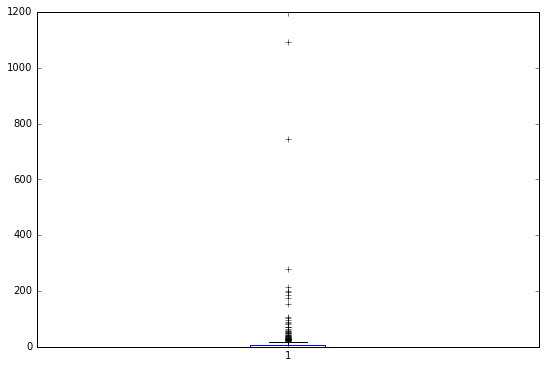
\includegraphics[width=65mm]{images/boxplots/area.png} &   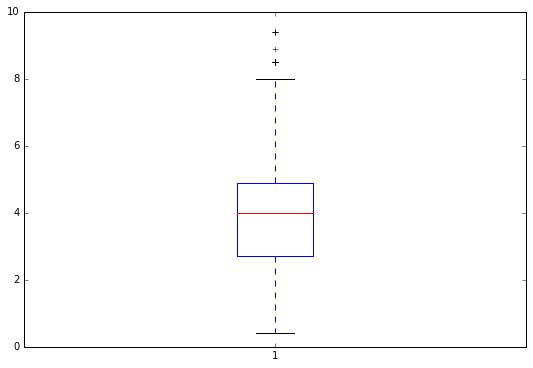
\includegraphics[width=65mm]{images/boxplots/wind.png} \\
(a) area & (b) wind \\[6pt]
 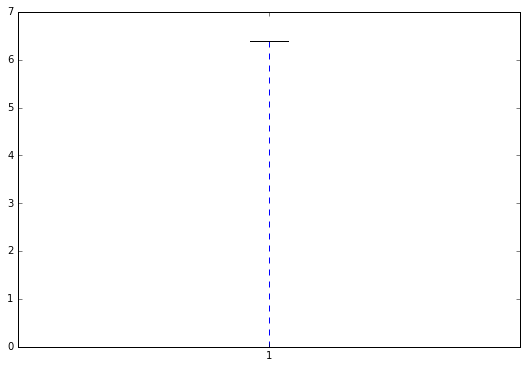
\includegraphics[width=65mm]{images/boxplots/rain.png} &   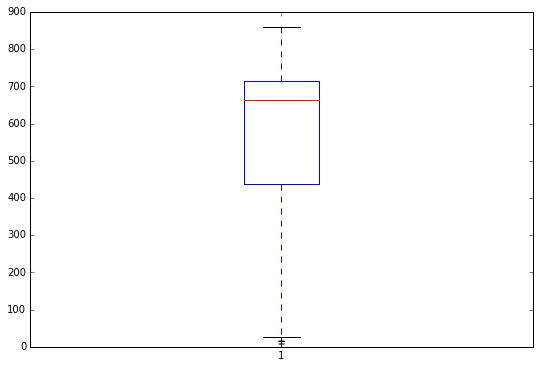
\includegraphics[width=65mm]{images/boxplots/DC.png} \\
(c) rain & (d) DC \\[6pt]
  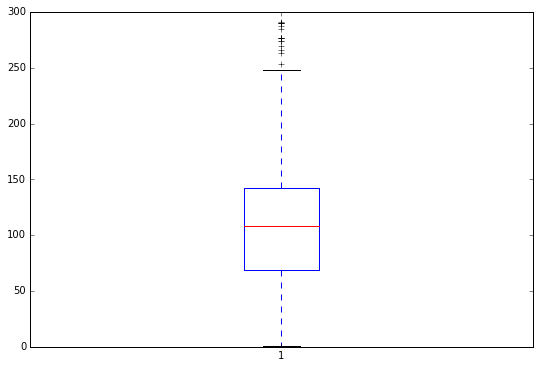
\includegraphics[width=65mm]{images/boxplots/DMC.png} &   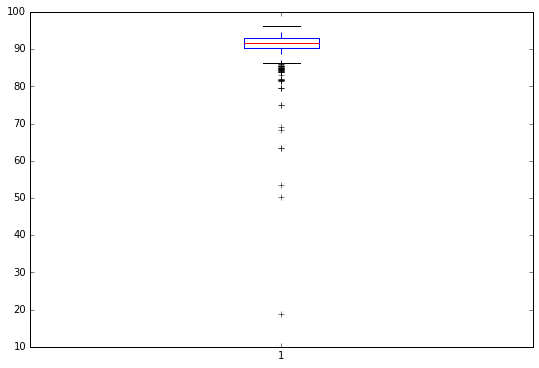
\includegraphics[width=65mm]{images/boxplots/FFMC.png} \\
(e) DMC & (f) FFMC \\[6pt]
\end{tabular}
\caption{Boxplot diagrams}
\end{figure}

\begin{figure}
\begin{tabular}{cc}
 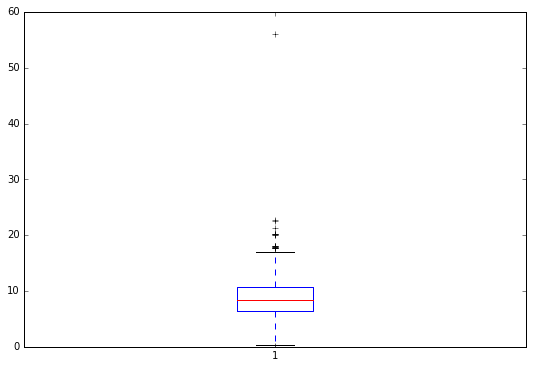
\includegraphics[width=65mm]{images/boxplots/ISI.png} &   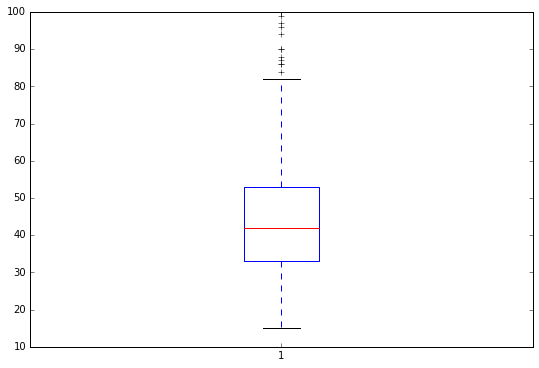
\includegraphics[width=65mm]{images/boxplots/RH.png} \\
(a) ISI & (b) RH \\[6pt]
  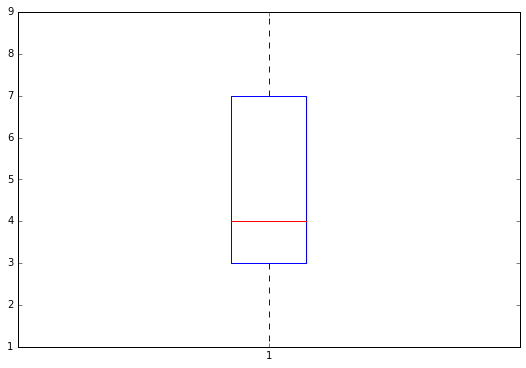
\includegraphics[width=65mm]{images/boxplots/x.png} &   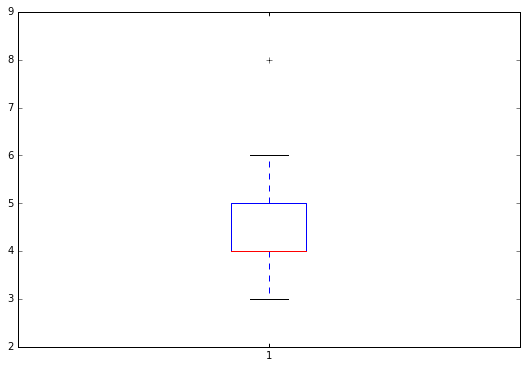
\includegraphics[width=65mm]{images/boxplots/y.png} \\
(c) X & (d) Y \\[6pt]
\multicolumn{2}{c}{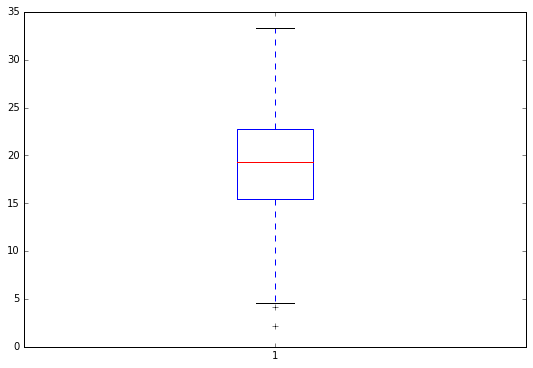
\includegraphics[width=65mm]{images/boxplots/temp.png} }\\
\multicolumn{2}{c}{(e) temp}
\end{tabular}
\caption{Boxplot diagrams}
\end{figure}